%%%%%%%%%%%%%%%%%%%%%%%%%%%%%%%%%%%%%%%%%%%%%%%%%%%%%%%%%%%%%%%%%%%%%%%%%%%%%%%%%%%%%%%%%%%%%%%%%%%%%%%%%
%%%%%  Topic 1 -- Cluster and Grid Computing                                                        %%%%%
%%%%%  Part of the Module 1 study material; compile main.tex for the full set,                      %%%%%
%%%%%  or this file on its own (it is a subfile and picks up ../preamble.tex).                      %%%%%
%%%%%%%%%%%%%%%%%%%%%%%%%%%%%%%%%%%%%%%%%%%%%%%%%%%%%%%%%%%%%%%%%%%%%%%%%%%%%%%%%%%%%%%%%%%%%%%%%%%%%%%%%
\documentclass[../main.tex]{subfiles}

\begin{document}


\topic{Cluster and Grid Computing}

\begin{tabularx}{\textwidth}{@{}>{\bfseries}p{3.4cm}L@{}}
\toprule
Course            & Modern Computing and Python Programming (26ESCC106) \\
Module            & Module 1 --- Modern Computing Approaches \\
Topic coverage    & Cluster and Grid Computing --- Introduction and Characteristics \\
Position in module& After Distributed Computing; before Cloud Computing \\
Mapped CO         & CO1 --- Describe modern computing approaches and their characteristics \\
Bloom's level     & L1 --- Remember, L2 --- Understand \\
Compiled by       & Mr. Manjunath Prasad H. R., Department of AI\&ML, MITE \\
Reviewed by       & \\
% Reviewed by       & 1.~Dr. Prashanth C. M., Principal, MITE\newline
%                     2.~Dr. Terrence Johnson, Professor and Associate Dean --- Academics\newline
%                     3.~Dr. Ravinarayana B., Professor and Head, Dept.\ of CS\&E \\
\bottomrule
\end{tabularx}


%%%%%%%%%%%%%%%%%%%%%%%%%%%%%%%%%%%%%%%%%%%%%%%%%%%%%%%%%%%%%%%%%%%%%%%%%%%%%%%%%%%%%%%%%%%%%
\section{Introduction}

The previous topic established that a distributed system is a collection of
independent computers that presents itself to its users as a single coherent
system~\rc{ref:buyya}. That definition permits many different arrangements, and the
differences between them matter. Two of these arrangements -- clusters and
grids -- are the subject of the topic in the module. They are important in
their own way, and they are also the foundation on which cloud computing, the next
topic in this module, is built.

Both answer the same question: how do you obtain more computing capacity than
one machine can provide? Their answers differ in one respect above all
others, and it is worth stating plainly at the outset because every other
difference follows from it.

\begin{notebox}
A cluster is many computers owned and administered by one organisation, in
one place, connected by a dedicated network. A grid is many computers owned
and administered by different organisations, in different places, connected
by the public network. Ownership is the distinction; everything else is a
consequence of it.
\end{notebox}


%%%%%%%%%%%%%%%%%%%%%%%%%%%%%%%%%%%%%%%%%%%%%%%%%%%%%%%%%%%%%%%%%%%%%%%%%%%%%%%%%%%%%%%%%%%%%
\section{Cluster Computing}

\subsection{Definition}

A computer cluster is a set of complete, standalone computers connected by a
dedicated high-speed local network and working together as a single
integrated computing resource~\rcc{ref:hwang}{ref:yeo}. Each machine in the cluster --- called a
node --- has its own processor, memory, storage and operating system, and
could function independently. What makes the collection a cluster is that
software coordinates the nodes so that a user submits work to the cluster as
a whole rather than to any particular machine.

Figure~\ref{fig:basic} illustrates the basic idea. The input data is given to
the root (master) node, which divides the work and distributes the parts to
the slave (worker) nodes. The nodes work on their parts in parallel and
exchange intermediate results with one another over the network where the
problem requires it. The root node then collects the partial results and
produces the final output.

\begin{figure}[!htb]
\centering
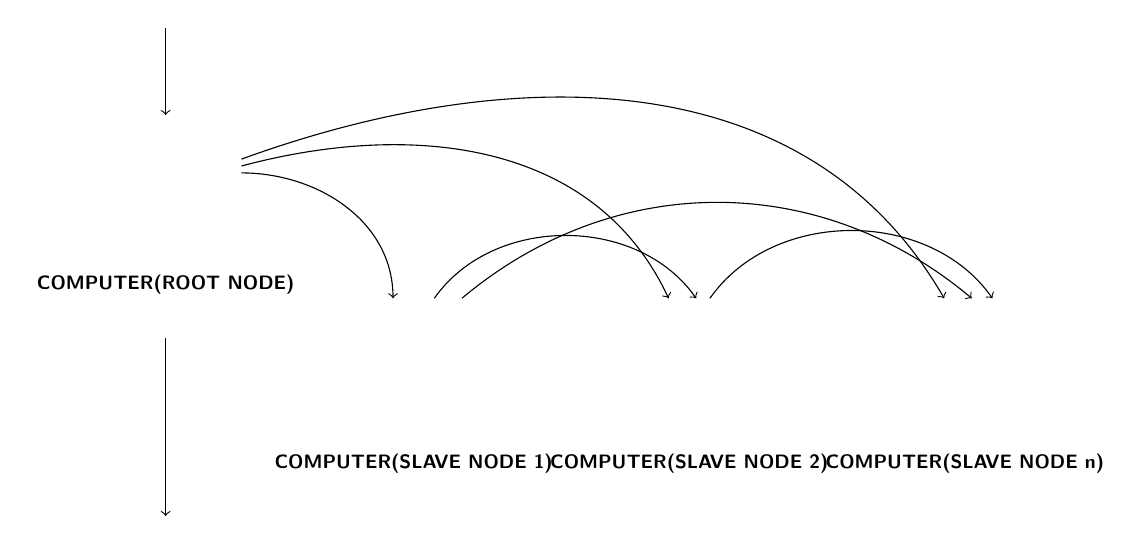
\begin{tikzpicture}[x=1.75cm,y=1.75cm]
  \tikzset{lbl/.append style={font=\sffamily\scriptsize\bfseries}}
  \B{0.1,4.1}{2.1,4.52}{INPUT DATA}
  \B{0.5,0.12}{1.7,0.54}{RESULTS}
  \monitor{1.1}{3.05}
  \node[lbl,anchor=north] at (1.1,2.38) {COMPUTER\\(ROOT NODE)};
  \draw[->] (1.1,4.1) -- (1.1,3.47);
  \draw[->] (1.1,1.85) -- (1.1,0.56);
  \foreach \x/\n in {2.9/1, 4.9/2, 6.9/n} {
    \monitor{\x}{1.75}
    \node[lbl,anchor=north] at (\x,1.08) {COMPUTER\\(SLAVE NODE \n)};
  }
  \draw[->] (1.65,3.05) to[out=0,in=90]   (2.75,2.14);
  \draw[->] (1.65,3.10) to[out=15,in=115] (4.75,2.14);
  \draw[->] (1.65,3.15) to[out=20,in=120] (6.75,2.14);
  \draw[->] (3.05,2.14) to[bend left=55] (4.95,2.14);
  \draw[->] (3.25,2.14) to[bend left=40] (6.95,2.14);
  \draw[->] (5.05,2.14) to[bend left=55] (7.10,2.14);
\end{tikzpicture}
\caption{Basic working model of cluster computing}
\label{fig:basic}
\end{figure}

\subsection{Why Clusters Exist}

Until the early 1990s, an organisation needing very high computational
capacity bought a supercomputer: a custom-designed machine with specially
built processors and memory systems, produced in small numbers and priced
accordingly. Meanwhile, mass-produced personal computer components were
improving rapidly and falling in price, precisely because they were
mass-produced.

The cluster is the consequence of noticing that a hundred ordinary machines
cost far less than one extraordinary machine of comparable aggregate
capacity. The idea was demonstrated in 1994 at NASA's Goddard Space Flight
Center, where Thomas Sterling and Donald Becker built a working parallel
machine from sixteen commodity personal computers and standard Ethernet
running free software. The arrangement became known as a Beowulf
cluster~\rc{ref:beowulf}, and it established that serious parallel computing did not require
specialised hardware.

The trade-off is real and should be understood. Commodity components are
cheap but their interconnect is slower relative to processor speed than in a
purpose-built supercomputer. A cluster therefore performs well on problems
that divide into parts needing little communication between them, and less
well on problems requiring constant exchange of intermediate results.

\subsection{Components of a Cluster}

\begin{center}
\begin{tabularx}{\textwidth}{@{}p{4.2cm}L@{}}
\toprule
\textbf{Component} & \textbf{Function} \\
\midrule
Compute nodes & Standalone computers that perform the actual work; each has
  its own processor, memory and operating system \\
Head or master node & The single point of entry through which users log in
  and submit work; it does not usually perform computation itself \\
High-speed interconnect & A dedicated private network joining the nodes ---
  typically 10-, 25- or 100-Gigabit Ethernet, or InfiniBand where very low
  latency is required \\
Cluster middleware & Software that makes the collection behave as one
  machine, providing the single system image and handling node failure \\
Resource manager and job scheduler & Accepts submitted jobs, queues them,
  allocates nodes and manages execution --- for example Slurm or PBS \\
Parallel programming environment & Libraries that let one program run across
  many nodes, most commonly MPI for communication between nodes and OpenMP
  within a node \\
Shared storage & A file system visible to every node, so that a job can read
  its input and write its output regardless of where it runs \\
\bottomrule
\end{tabularx}
\end{center}

\subsection{Cluster Architecture}

Figure~\ref{fig:arch} shows the generic architecture of a cluster, as
presented by Yeo, Buyya \emph{et al.}~\rc{ref:yeo}. It is read from the
bottom up. The
nodes --- PCs or workstations --- are joined by the cluster interconnection
network or switch. Each node has network interface hardware that attaches it
to this network, communication software that provides fast and reliable data
exchange between nodes, and its own operating system. Above the individual
nodes sits the cluster middleware, which provides the single system image and
the availability infrastructure: it makes the separate machines appear as one
computer and keeps the service running when a node fails. On top of the
middleware, sequential applications run directly, while parallel applications
run through a parallel programming environment --- compilers, message-passing
libraries such as MPI, debuggers and performance tools --- that lets one
program use many nodes at once.

\begin{figure}[!htb]
\centering
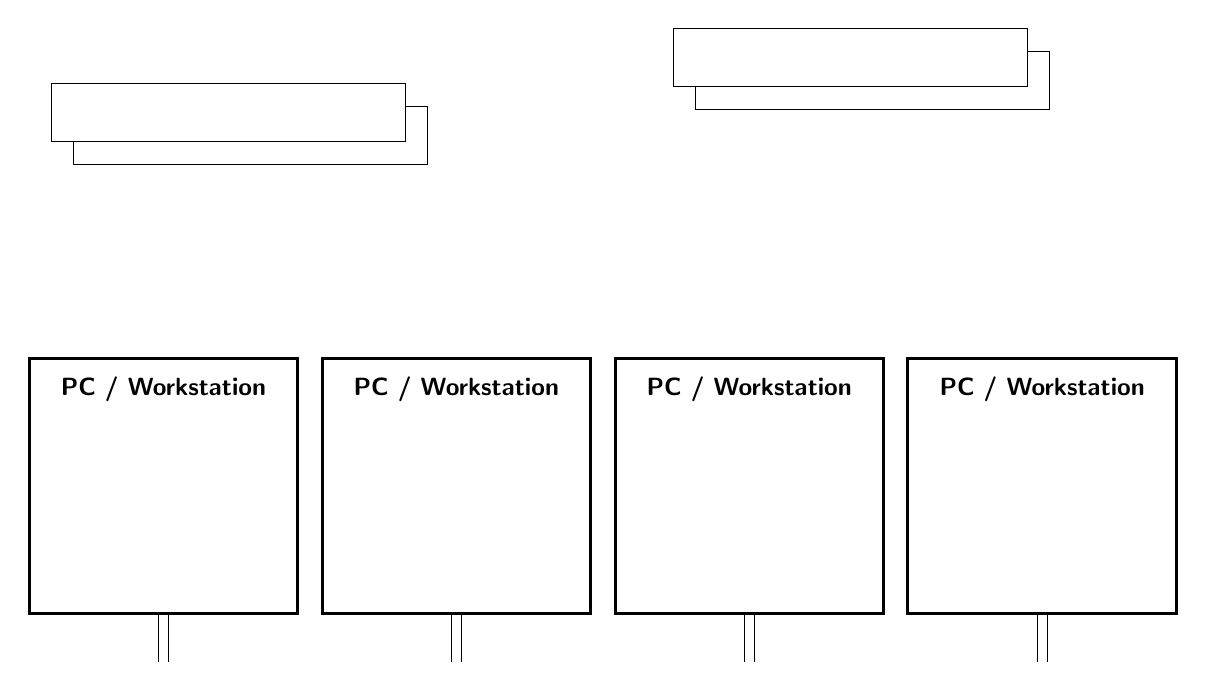
\begin{tikzpicture}[x=1.55cm,y=1.75cm]
  \tikzset{lbl/.append style={font=\sffamily\small\bfseries}}
  \foreach \k in {2,1} {
    \draw[fill=white] (0.3+0.18*\k,4.55-0.17*\k) rectangle ++(2.9,0.42);
    \draw[fill=white] (5.4+0.18*\k,4.95-0.17*\k) rectangle ++(2.9,0.42);
  }
  \B[fill=white]{0.3,4.55}{3.2,4.97}{Sequential Applications}
  \B[fill=white]{5.4,4.95}{8.3,5.37}{Parallel Applications}
  \B{4.3,3.95}{9.7,4.40}{Parallel Programming Environment}
  \B[line width=1.2pt]{0.3,3.0}{9.7,3.7}{Cluster Middleware\\(Single System Image and Availability Infrastructure)}
  \foreach \x in {0.3,2.7,5.1,7.5} {
    \draw[line width=1.1pt] (\x,0.95) rectangle ++(2.2,1.85);
    \node[lbl] at (\x+1.1,2.58) {PC / Workstation};
    \B{\x+0.15,2.10}{\x+2.05,2.40}{\mdseries\scriptsize Operating System}
    \B{\x+0.15,1.55}{\x+2.05,2.00}{\mdseries\scriptsize Communication\\\mdseries\scriptsize Software}
    \B{\x+0.15,1.05}{\x+2.05,1.45}{\mdseries\scriptsize Network Interface\\\mdseries\scriptsize Hardware}
    \draw (\x+1.06,0.95) -- (\x+1.06,0.60);
    \draw (\x+1.14,0.95) -- (\x+1.14,0.60);
  }
  \B[line width=1.2pt]{0.3,0.15}{9.7,0.60}{Cluster Interconnection Network / Switch}
\end{tikzpicture}
\caption{Cluster computer architecture (redrawn from~\rc{ref:yeo}; the figure originates in~\rc{ref:hpcc})}
\label{fig:arch}
\end{figure}

Figure~\ref{fig:physical} shows how such a cluster is typically deployed in
practice. Users never connect to the compute nodes directly; they log in to
the head node over the campus network or the Internet and submit their jobs
to the scheduler running there. The head node, the shared storage and every
compute node are joined by the private high-speed interconnect, which carries
the messages exchanged between the parts of a running job as well as the
traffic between each node and the shared file system. The head node and the
shared storage are where much of the middleware and scheduling software of
Figure~\ref{fig:arch} actually runs. Everything inside the dashed boundary
belongs to one organisation and sits in one facility.

\begin{figure}[!htb]
\centering
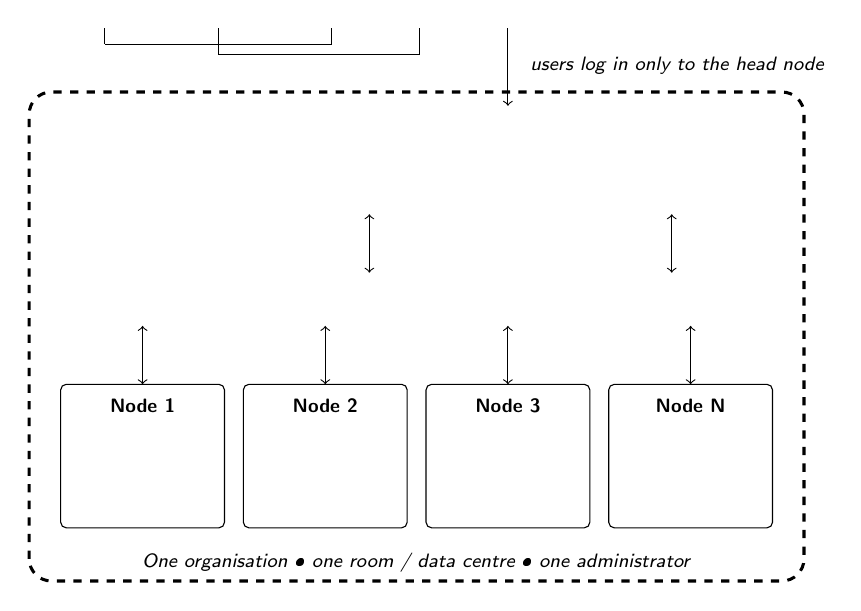
\begin{tikzpicture}[x=1.6cm,y=1.35cm,rounded corners=2pt]
  \tikzset{lbl/.append style={font=\sffamily\scriptsize}}
  % users and network
  \foreach \i in {0,1,2}
    \B{0.3+0.9*\i,5.35}{1.1+0.9*\i,5.77}{User \the\numexpr\i+1\relax};
  \B[dashed]{3.2,5.35}{5.4,5.77}{Campus network / Internet}
  \foreach \x in {0.7,1.6,2.5} \draw[sharp corners] (\x,5.35) -- (\x,5.2);
  \draw[sharp corners] (0.7,5.2) -- (2.5,5.2);
  \draw[sharp corners] (1.6,5.2) -- (1.6,5.1) -- (3.2,5.1) -- (3.2,5.35);
  \draw[->] (3.9,5.35) -- (3.9,4.62);
  \node[lbl,anchor=west,font=\sffamily\scriptsize\itshape] at (4.0,5.0) {users log in only to the head node};
  % cluster boundary
  \draw[dashed,line width=1.1pt,rounded corners=8pt] (0.1,0.15) rectangle (6.25,4.75);
  \node[lbl,font=\sffamily\scriptsize\itshape] at (3.17,0.32)
    {One organisation \textbullet{} one room / data centre \textbullet{} one administrator};
  \B{1.45,3.6}{4.15,4.6}{\textbf{Head (master) node}\\login, job submission\\resource manager\\and scheduler}
  \B{4.35,3.6}{6.05,4.6}{\textbf{Shared storage}\\(file system seen\\by every node)}
  \B[line width=1.1pt]{0.35,2.55}{6.0,3.05}{\textbf{High-speed private interconnect}\\(Ethernet / InfiniBand switch)}
  \draw[<->] (2.8,3.6) -- (2.8,3.05);
  \draw[<->] (5.2,3.6) -- (5.2,3.05);
  \foreach \x/\n in {0.35/1, 1.8/2, 3.25/3, 4.7/N} {
    \draw (\x,0.65) rectangle ++(1.3,1.35);
    \node[lbl,font=\sffamily\scriptsize\bfseries] at (\x+0.65,1.8) {Node \n};
    \B{\x+0.1,1.33}{\x+1.2,1.57}{\tiny CPU + memory}
    \B{\x+0.1,1.03}{\x+1.2,1.27}{\tiny own OS}
    \B{\x+0.1,0.73}{\x+1.2,0.97}{\tiny local disk}
    \draw[<->] (\x+0.65,2.0) -- (\x+0.65,2.55);
  }
\end{tikzpicture}
\caption{Physical organisation of a cluster}
\label{fig:physical}
\end{figure}

\subsection{Single System Image}

The property that distinguishes a cluster from a merely networked room of
computers is the single system image: the cluster presents itself to the user
as one machine. The user does not choose which nodes will run their program,
does not log in to individual machines, and does not manually distribute
data. They describe the resources their job needs and submit it; the
scheduler decides where it runs. This abstraction is what makes a cluster
usable, and providing it is the main job of the cluster
middleware~\rcc{ref:yeo}{ref:hwang}.

\subsection{Characteristics of Cluster Computing}
The following are the characteristics of cluster computing:
\begin{itemize}
  \item \textbf{Single administrative domain} --- all nodes are owned, funded
        and administered by one organisation, under one security policy
  \item \textbf{Physical co-location} --- nodes sit in one room or one data
        centre, typically in the same rack or set of racks
  \item \textbf{Homogeneity} --- nodes are usually identical or near-identical
        in hardware, operating system and configuration, which simplifies
        scheduling and programming
  \item \textbf{Tight coupling} --- a dedicated, private, high-bandwidth and
        low-latency interconnect, not shared with general network traffic
  \item \textbf{Dedicated resources} --- nodes exist to serve the cluster and
        are not used for anything else
  \item \textbf{Centralised scheduling} --- one resource manager has complete
        knowledge of and authority over every node
  \item \textbf{Single system image} --- the collection appears to the user as
        one computer
  \item \textbf{High availability} --- the failure of one node need not stop
        the cluster, because work can be restarted elsewhere
  \item \textbf{Incremental scalability} --- capacity grows by adding nodes,
        within the limits of space, power and interconnect
\end{itemize}

\subsection{Types of Clusters}

Clusters are built for three broad purposes~\rc{ref:hwang}.

\begin{center}
\begin{tabularx}{\textwidth}{@{}p{3.6cm}LL@{}}
\toprule
\textbf{Type} & \textbf{Purpose} & \textbf{Typical use} \\
\midrule
High-performance (HPC) cluster & Maximise computational throughput on a
  single large problem by dividing it across nodes & Scientific simulation,
  weather modelling, molecular dynamics, model training \\
Load-balancing cluster & Distribute many independent incoming requests
  across nodes so that no node is overwhelmed & Web servers, application
  servers, online services \\
High-availability (failover) cluster & Maintain service continuity by having
  standby nodes take over when an active node fails & Database servers,
  banking and other systems that must not stop \\
\bottomrule
\end{tabularx}
\end{center}

\subsection{Examples of Clusters}

\begin{itemize}
  \item Beowulf clusters --- the original 1994 NASA machine and the many
        university and departmental clusters modelled on it, built from
        commodity PCs running Linux
  \item The PARAM series developed by C-DAC under the National
        Supercomputing Mission, for example PARAM Siddhi-AI at C-DAC Pune and
        PARAM Pravega at IISc Bengaluru --- high-performance clusters of many
        compute nodes joined by a high-speed interconnect~\rc{ref:cdac}
  \item Most of the world's fastest computers listed in the TOP500 ranking,
        which are built as clusters rather than as single custom
        machines~\rc{ref:top500}
  \item Web server farms behind a load balancer --- search engines,
        e-commerce and railway or airline booking sites spread incoming
        requests across many identical servers (load-balancing clusters)
  \item High-availability database clusters, such as Oracle Real Application
        Clusters, used for core banking and reservation systems where a
        standby node must take over if an active node fails
\end{itemize}

\subsection{Advantages and Limitations}

\textbf{Advantages}
\begin{itemize}
  \item Substantially better price-to-performance ratio than a purpose-built
        supercomputer
  \item Capacity can be increased in small increments rather than by
        replacing the whole machine
  \item Redundancy is inherent, so availability is high if the software is
        configured for it
  \item Built from standard components with standard software, so expertise
        and spare parts are widely available
\end{itemize}

\textbf{Limitations}
\begin{itemize}
  \item Bounded by one organisation's budget, floor space, power supply and
        cooling capacity
  \item Programs must be written explicitly for parallel execution; existing
        sequential software does not benefit
  \item The interconnect eventually limits how far a tightly coupled problem
        can be scaled
  \item Capacity is fixed once purchased --- it must be sized for peak demand
        and is idle at other times
\end{itemize}

%%%%%%%%%%%%%%%%%%%%%%%%%%%%%%%%%%%%%%%%%%%%%%%%%%%%%%%%%%%%%%%%%%%%%%%%%%%%%%%%%%%%%%%%%%%%%
\section{Grid Computing}

\subsection{Definition}

Grid computing is the coordinated sharing of computing resources that belong
to different organisations, in different locations, in order to solve a
common problem. The resources are federated rather than owned in common: each
participating institution keeps ownership of and authority over its own
machines, and contributes their use under agreed terms.

The term was introduced in the late 1990s, principally through the work of
Ian Foster and Carl Kesselman~\rc{ref:blueprint}, who characterised the field
by the problem of coordinated resource sharing across institutional
boundaries~\rc{ref:anatomy}.

\subsection{The Power Grid Analogy}

The name is borrowed from the electrical power grid, and the analogy explains
the ambition~\rc{ref:blueprint}. When you switch on a light, you do not know or care which
generating station supplied the electricity, whether it came from one source
or several, or where those sources are. You draw power from a socket, it is
metered, and you are billed. The generation, transmission and coordination
are invisible.

Grid computing proposed the same relationship with computation: a researcher
would draw processing power from a socket without knowing which
institution's machines were serving them. It is worth noting that this
ambition was only partially realised. Electricity is a uniform commodity and
computing is not --- machines differ in architecture, software and policy in
ways that generators do not --- and the seamlessness the analogy promised
proved difficult to deliver. The vision was largely fulfilled later, by cloud
computing, and by a different route.

\subsection{The Virtual Organisation}

The central concept in grid computing is the virtual organisation: a set of
individuals or institutions, drawn from different real organisations, who
agree to share specified resources under specified rules for a specified
purpose. A virtual organisation is defined by its sharing agreement, not by a
legal entity or a physical site~\rc{ref:anatomy}.

A concrete example makes this clear. Physicists at twenty universities in
twelve countries collaborate on one experiment. Each university owns a
cluster. No university is willing to hand over control of its cluster to any
other, and each has its own security policy, its own users and its own local
commitments. Yet the experiment needs more capacity than any one of them has.
The virtual organisation is the arrangement under which those twenty clusters
serve the experiment while each remains under its owner's control. Grid
middleware exists to make that arrangement work in practice.

\subsection{Grid Architecture}

Figure~\ref{fig:grid} shows how the sites of a grid are arranged and how a
user's job reaches them. Each site --- a university cluster, a research
laboratory's supercomputer, a data archive, a scientific instrument, or a pool
of contributed desktop PCs --- is owned by a different institution. Every site
keeps its own local scheduler and its own policy, which decide what may run
there, for whom and at what priority; nothing in the grid overrides them. A
layer of grid middleware at each site acts as a gateway, translating a request
arriving from the grid into a local action that the owner has already agreed
to permit. The sites are joined only by the wide-area network, drawn in the
middle of the figure, and the dashed boundary around them is the virtual
organisation: an agreement, not a building or a company.

The upper part of the figure shows what happens when work is submitted. The
user does not approach the sites one by one. They authenticate once with a
digital certificate and hand the job to a grid portal or resource broker,
which is the only component they deal with directly. The broker asks the
information service which resources are currently available and suitable ---
what exists, what is free, and what matches the job's requirements --- because
membership of a grid changes without notice. The security service then
establishes that this user, authenticated at their home institution, is to be
trusted at each site the broker has chosen, so that one login is accepted
everywhere (single sign-on). Only then does the broker dispatch the job, and
the data it needs, across the network. At the receiving site the middleware
hands the job to the local scheduler, which queues it like any local work, and
the results travel back the same way. Everything the user would otherwise have
to do --- find resources, negotiate access at each institution, move data,
track progress --- is what the middleware and these services exist to do.

\begin{figure}[!htb]
\centering
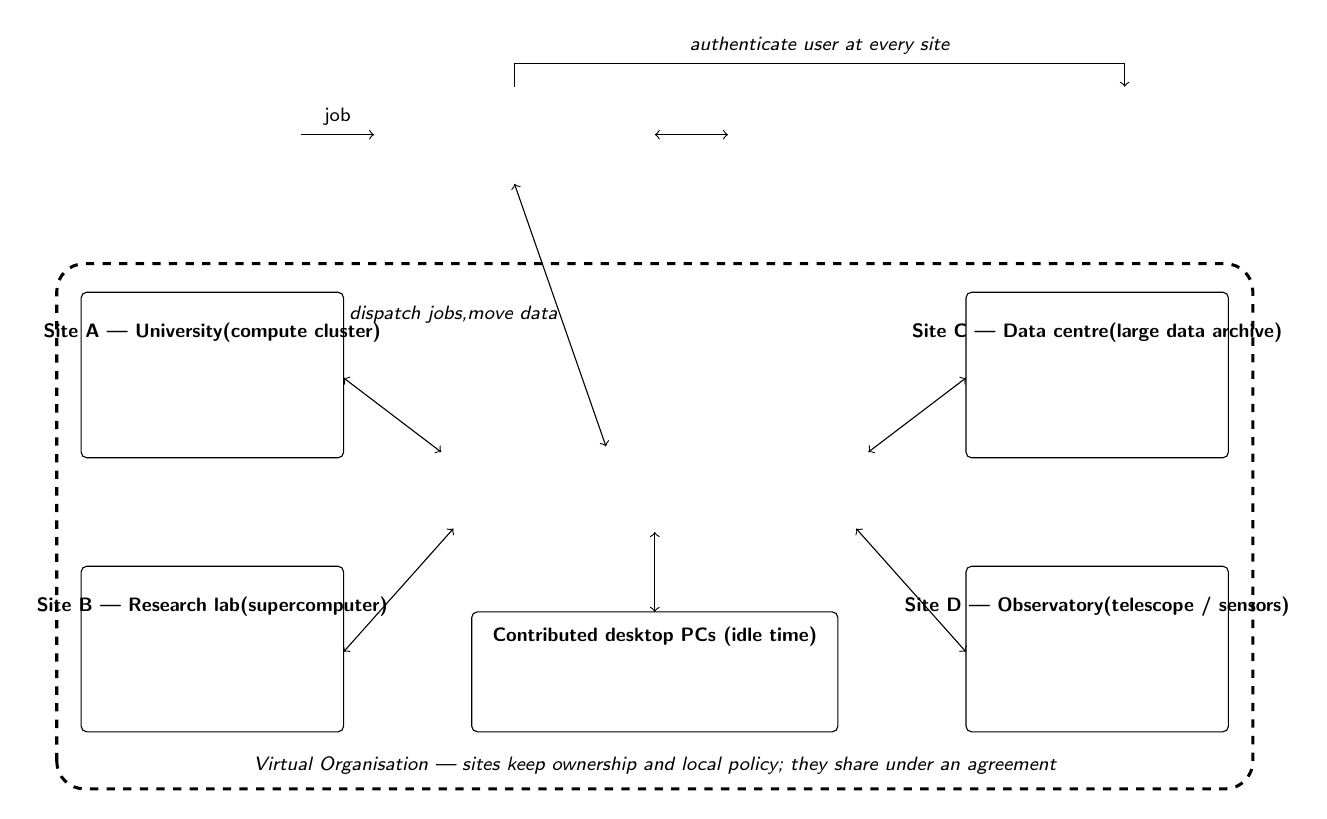
\begin{tikzpicture}[x=1.55cm,y=1.45cm,rounded corners=2pt]
  \tikzset{lbl/.append style={font=\sffamily\scriptsize}}
  % services
  \B{0.3,5.35}{2.1,6.2}{User\\(with grid\\certificate)}
  \B{2.7,5.35}{5.0,6.2}{\textbf{Grid portal /}\\\textbf{resource broker}}
  \B{5.6,5.35}{7.5,6.2}{Information service\\(resource\\discovery)}
  \B{7.9,5.35}{9.8,6.2}{Security service\\(single sign-on,\\trust between sites)}
  \draw[->] (2.1,5.78) -- node[lbl,above]{job} (2.7,5.78);
  \draw[<->] (5.0,5.78) -- (5.6,5.78);
  \draw[->,sharp corners] (3.85,6.2) -- (3.85,6.4) -- node[lbl,above,font=\sffamily\scriptsize\itshape]{authenticate user at every site} (8.85,6.4) -- (8.85,6.2);
  % virtual organisation boundary
  \draw[dashed,line width=1.1pt,rounded corners=10pt] (0.1,0.05) rectangle (9.9,4.65);
  \node[lbl,font=\sffamily\scriptsize\itshape] at (5,0.25)
    {Virtual Organisation --- sites keep ownership and local policy; they share under an agreement};
  % wide-area network
  \B[dashed,rounded corners=12pt]{3.0,2.3}{7.0,3.05}{Wide-area network / Internet\\(shared, high latency)}
  \draw[<->] (3.85,5.35) -- (4.6,3.05);
  \node[lbl,font=\sffamily\scriptsize\itshape] at (3.35,4.2) {dispatch jobs,\\move data};
  % sites
  \foreach \x/\y/\t in {0.3/2.95/{Site A --- University\\(compute cluster)},
                        0.3/0.55/{Site B --- Research lab\\(supercomputer)},
                        7.55/2.95/{Site C --- Data centre\\(large data archive)},
                        7.55/0.55/{Site D --- Observatory\\(telescope / sensors)}} {
    \draw (\x,\y) rectangle ++(2.15,1.45);
    \node[lbl,font=\sffamily\scriptsize\bfseries] at (\x+1.075,\y+1.1) {\t};
    \B{\x+0.12,\y+0.48}{\x+2.03,\y+0.78}{\tiny grid middleware (gateway)}
    \B{\x+0.12,\y+0.10}{\x+2.03,\y+0.40}{\tiny local scheduler \& policy}
  }
  \draw[<->] (2.45,3.65) -- (3.25,3.0);
  \draw[<->] (2.45,1.25) -- (3.35,2.33);
  \draw[<->] (7.55,3.65) -- (6.75,3.0);
  \draw[<->] (7.55,1.25) -- (6.65,2.33);
  \draw (3.5,0.55) rectangle (6.5,1.6);
  \node[lbl,font=\sffamily\scriptsize\bfseries] at (5,1.38) {Contributed desktop PCs (idle time)};
  \foreach \i in {0,...,3} \B{3.82+0.62*\i,0.7}{4.32+0.62*\i,1.05}{\tiny PC};
  \draw[<->] (5,1.6) -- (5,2.3);
\end{tikzpicture}
\caption{Architecture of a grid --- independent sites joined into a virtual
organisation through grid middleware}
\label{fig:grid}
\end{figure}

Internally, this software is organised in layers~\rc{ref:anatomy}. The Fabric
layer is the physical resources themselves, each under its local manager. The
Connectivity layer provides communication and security between sites. The
Resource layer negotiates access to, and controls, one resource at a time,
such as starting and monitoring a job on one cluster. The Collective layer
coordinates many resources together --- discovery, brokering, scheduling
across sites and monitoring --- and it is where the information service and
the resource broker of Figure~\ref{fig:grid} belong. Applications sit on top
and use these services. The Globus Toolkit provided software for the
Connectivity, Resource and Collective layers.

\subsection{Characteristics of Grid Computing}

\begin{itemize}
  \item \textbf{Multiple administrative domains} --- no single owner or
        authority; each site retains autonomy over its own resources and
        enforces its own policies
  \item \textbf{Geographical distribution} --- resources are spread across
        cities, countries or continents
  \item \textbf{Heterogeneity} --- nodes differ in hardware architecture,
        operating system, software stack and configuration
  \item \textbf{Loose coupling} --- sites are connected by wide-area networks
        or the public Internet, with latency orders of magnitude higher than a
        cluster interconnect
  \item \textbf{Dynamic and unpredictable membership} --- resources join,
        leave and fail without notice, so the grid must tolerate their
        disappearance
  \item \textbf{Non-dedicated resources} --- contributed machines usually
        have local work of their own, and grid jobs run on spare capacity at
        lower priority
  \item \textbf{Policy-based sharing} --- what may be used, by whom, and for
        what is governed by negotiated agreements rather than by ownership
  \item \textbf{Decentralised scheduling} --- no single scheduler has
        authority over all resources; allocation is negotiated between sites
  \item \textbf{Reliance on standard protocols and middleware} --- the Globus
        Toolkit and the Open Grid Services Architecture were the principal
        efforts to standardise this
  \item \textbf{Best-effort service} --- there is generally no guarantee of
        when a job will run or on what, because no participant has undertaken
        to provide capacity on demand
\end{itemize}

\subsection{Types of Grids}

Grids are classified by what they share~\rcc{ref:hwang}{ref:blueprint}.

\begin{center}
\begin{tabularx}{\textwidth}{@{}p{4.2cm}L@{}}
\toprule
\textbf{Type} & \textbf{Description} \\
\midrule
Computational grid & Aggregates processing capacity across sites to execute
  computationally intensive work \\
Data grid & Provides controlled, coordinated access to very large datasets
  held at multiple institutions \\
Collaboration or service grid & Shares instruments, services and
  applications --- telescopes, sensors, specialised software --- rather than
  raw computation \\
Desktop or volunteer grid & Uses idle time on ordinary personal computers
  contributed by the public, coordinated over the Internet \\
\bottomrule
\end{tabularx}
\end{center}

\subsection{Examples}

\begin{itemize}
  \item The Worldwide LHC Computing Grid, which distributes and processes
        data from the Large Hadron Collider across roughly 170 computing
        centres in more than 40 countries~\rc{ref:wlcg}
  \item The European Grid Infrastructure, federating computing resources
        across European research institutions~\rc{ref:egi}
  \item GARUDA, the Indian national grid initiative coordinated by C-DAC,
        connecting research and academic institutions across the
        country~\rc{ref:cdac}
  \item Volunteer computing projects for protein folding and radio-signal
        analysis, run on donated capacity from personal computers
\end{itemize}

\subsection{Advantages and Limitations}

\textbf{Advantages}
\begin{itemize}
  \item Exploits existing resources that would otherwise sit idle, at little
        additional hardware cost
  \item Aggregate capacity far exceeding what any single participant could
        afford to build
  \item Enables collaboration across institutional and national boundaries
        without transferring ownership
  \item No participant is required to purchase the whole of the capacity it
        occasionally needs
\end{itemize}

\textbf{Limitations}
\begin{itemize}
  \item Heterogeneity makes software difficult to write, deploy and validate
        across sites
  \item Security and trust are hard: a user authenticated at one institution
        must be granted appropriate rights at another that does not directly
        know them
  \item Wide-area latency makes the grid unsuitable for tightly coupled
        problems requiring frequent communication
  \item Middleware is complex and demands specialist administration at every
        participating site
  \item No guarantee of availability or performance, because resources are
        contributed rather than committed
  \item Accounting is difficult --- measuring and settling who consumed whose
        capacity never worked cleanly, which limited participation beyond
        publicly funded research
\end{itemize}

%%%%%%%%%%%%%%%%%%%%%%%%%%%%%%%%%%%%%%%%%%%%%%%%%%%%%%%%%%%%%%%%%%%%%%%%%%%%%%%%%%%%%%%%%%%%%
\section{Cluster Computing versus Grid Computing}

The table below draws together the differences established in the two
previous sections~\rcc{ref:hwang}{ref:anatomy}.

\begin{center}
\begin{tabularx}{\textwidth}{@{}p{3.2cm}LL@{}}
\toprule
\textbf{Aspect} & \textbf{Cluster computing} & \textbf{Grid computing} \\
\midrule
Ownership & One organisation & Many independent organisations \\
Administration & Single administrative domain & Multiple autonomous domains \\
Location & Co-located in one facility & Geographically distributed \\
Hardware and software & Homogeneous & Heterogeneous \\
Interconnect & Dedicated high-speed LAN, low latency & Wide-area network or
  Internet, high latency \\
Coupling & Tight & Loose \\
Resource dedication & Dedicated to the cluster & Shared with the owner's own
  local workload \\
Scheduling & Centralised, with full authority & Decentralised and
  negotiated \\
Membership & Static and known & Dynamic and variable \\
Security & One policy, one trust domain & Cross-domain trust and identity
  federation required \\
Service guarantee & Predictable and controlled & Best effort \\
User view & A single machine & A pool of resources reached through
  middleware \\
Suitable workload & Tightly coupled parallel problems & Independent,
  coarse-grained tasks \\
\bottomrule
\end{tabularx}
\end{center}

%%%%%%%%%%%%%%%%%%%%%%%%%%%%%%%%%%%%%%%%%%%%%%%%%%%%%%%%%%%%%%%%%%%%%%%%%%%%%%%%%%%%%%%%%%%%%
\section{Review Questions}

\textbf{CO1 --- Describe modern computing approaches and their
characteristics}\\
\textit{Bloom's Level L1 --- Remember, L2 --- Understand}

\begin{enumerate}[label=\arabic*.]
  \item Define cluster computing and explain what distinguishes a cluster
        from a set of networked computers in the same room.
  \item List the principal components of a cluster and state the function of
        each.
  \item Explain the term single system image and describe why it matters to
        a cluster user.
  \item List any six characteristics of cluster computing.
  \item With a neat diagram, explain the architecture of a computer cluster,
        showing both its physical organisation and its software layers.
  \item With a neat diagram, explain how a user's job is executed on a grid,
        stating the role of the resource broker, the information service, the
        security service and the grid middleware at each site.
  \item Differentiate between high-performance, load-balancing and
        high-availability clusters, giving one application of each.
  \item State any four limitations of cluster computing.
  \item Explain the power grid analogy. Identify one respect in which the
        analogy does not hold.
  \item What is a virtual organisation? Explain with an example why it is the
        central concept in grid computing.
  \item List any six characteristics of grid computing.
  \item Differentiate between a computational grid and a data grid.
  \item Compare cluster and grid computing with respect to ownership,
        coupling, homogeneity, scheduling and service guarantee.
  \item Explain why security is substantially harder to provide in a grid
        than in a cluster.
  \item Why is grid computing unsuitable for tightly coupled parallel
        problems?
  \item Give one real-world example each of a high-performance, a
        load-balancing and a high-availability cluster.

\end{enumerate}

%%%%%%%%%%%%%%%%%%%%%%%%%%%%%%%%%%%%%%%%%%%%%%%%%%%%%%%%%%%%%%%%%%%%%%%%%%%%%%%%%%%%%%%%%%%%%
\section{References and Further Reading}

Items~\ref{ref:hwang} to~\ref{ref:hpcc} are the sources used in preparing
these notes and are suggested for further reading; section and chapter
numbers are indicative. Items~\ref{ref:wlcg} to~\ref{ref:cdac} are the
project and ranking sites from which the examples and figures quoted in the
text were taken.

\begin{enumerate}[label={[\arabic*]},ref=\arabic*,leftmargin=2.2em]
  \item\label{ref:hwang} K.~Hwang, G.~C.~Fox and J.~J.~Dongarra,
        \textit{Distributed and Cloud Computing: From Parallel Processing to
        the Internet of Things}, Morgan Kaufmann, 2012 --- Chapter~2 on
        computer clusters for scalable parallel computing, and Chapter~7 on
        grid computing systems and resource management.
  \item\label{ref:buyya} R.~Buyya, C.~Vecchiola, S.~T.~Selvi, S.~Poojara and
        S.~N.~Srirama, \textit{Mastering Cloud Computing}, 2nd Edition,
        Morgan Kaufmann, 2026 --- Chapter~2 on the principles of parallel and
        distributed computing.
  \item\label{ref:yeo} C.~S.~Yeo, R.~Buyya, H.~Pourreza, R.~Eskicioglu,
        P.~Graham and F.~Sommers, ``Cluster Computing: High-Performance,
        High-Availability, and High-Throughput Processing on a Network of
        Computers'', in A.~Y.~Zomaya (ed.), \textit{Handbook of
        Nature-Inspired and Innovative Computing}, Springer, 2006 --- the
        source of Figure~\ref{fig:arch}.
  \item\label{ref:beowulf} T.~Sterling, D.~J.~Becker, D.~Savarese,
        J.~E.~Dorband, U.~A.~Ranawake and C.~V.~Packer, ``BEOWULF: A Parallel
        Workstation for Scientific Computation'', \textit{Proceedings of the
        24th International Conference on Parallel Processing}, 1995.
  \item\label{ref:blueprint} I.~Foster and C.~Kesselman (eds.), \textit{The
        Grid: Blueprint for a New Computing Infrastructure}, 2nd Edition,
        Morgan Kaufmann, 2004.
  \item\label{ref:anatomy} I.~Foster, C.~Kesselman and S.~Tuecke, ``The
        Anatomy of the Grid: Enabling Scalable Virtual Organizations'',
        \textit{International Journal of High Performance Computing
        Applications}, vol.~15, no.~3, pp.~200--222, 2001 --- the source of
        the virtual organisation and of the layered grid architecture.
  \item\label{ref:hpcc} R.~Buyya (ed.), \textit{High Performance Cluster
        Computing: Architectures and Systems}, Volume~1, Prentice Hall PTR,
        1999 --- where the architecture of Figure~\ref{fig:arch} first
        appeared.
  \item\label{ref:wlcg} Worldwide LHC Computing Grid, CERN.
        \url{https://wlcg.web.cern.ch/}
  \item\label{ref:egi} EGI Federation (European Grid Infrastructure).
        \url{https://www.egi.eu/}
  \item\label{ref:top500} TOP500 list of the world's most powerful computer
        systems. \url{https://www.top500.org/}
  \item\label{ref:cdac} Centre for Development of Advanced Computing (C-DAC)
        --- PARAM systems under the National Supercomputing Mission, and the
        GARUDA national grid initiative. \url{https://www.cdac.in/}
\end{enumerate}

\end{document}
